\begin{frame}
  \frametitle{Prossimi passi}
  \begin{columns}
    \column{0.5\textwidth}
    \begin{figure}[!htb]
      \centering
      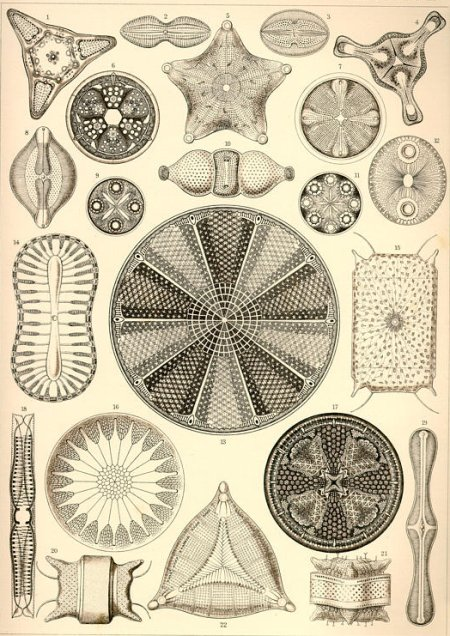
\includegraphics[width=0.9\textwidth]{../img/haeckel-diatoms}
    \end{figure}
    (Haeckel)
    \column{0.5\textwidth}
    \begin{itemize}
      \item Riprodurre risultati con lagrangiano parallelo
        \\
        (e maggiore dettaglio)
      \item Coesistenza di due o più popolazioni
    \end{itemize}
  \end{columns}

\end{frame}
